The equation for frequency response of a discrete-time linear
time-invariant system (Equation \ref{eq:dt_fr}) is also known as the
\emph{\index{Discrete-Time Fourier Transform}{Discrete-Time Fourier Transform}} (DTFT).
We can obtain a DTFT for an arbitrary discrete-time signal $x[n]$ as
follows\sidenote{Hat on top of $\hat{x}$ to signify that it is a
frequency domain representation of signal $x[n]$, and a hat on top of
$\hat{\omega}$ to signify that the frequency has units of radians per
sample.}:
\begin{equation}
\boxed{
\hat{x}(\hat{\omega}) = \sum_{n=-\infty}^{\infty} x[n] e^{-i\hat{\omega} n}\,\,.
}
\label{eq:dtft_eq}
\end{equation}
Here $\hat{x}(\hat{\omega})$ is the DTFT of a discrete-time signal
$x[n]$. We'll use the following notation for denoting DTFT pairs:
\begin{equation}
\boxed{
x[n] \xleftrightarrow{\mathcal{F}} \hat{x}(\hat{\omega})
}
\end{equation}
like we did in the Fourier transform chapter. The left-hand side
denotes the time domain representation, and the right-hand side
denotes the frequency domain representation.

Let's show that Equation \ref{eq:dtft_eq} is a special case of the
continuous-time Fourier transform for discretized signals. Remember
that the formula for discretizing a continuous-time signal is:
\begin{equation}
x[n] = x(nT_s)\,\,.%\int_{-\infty}^{\infty} \delta(t-n T_s) x(t) dt.
\end{equation}
Here $T_s$ is the sample spacing, which is related to sample-rate
$f_s=1/T_s$. The continuous-time representation of the discretized
signal is defined as:
\begin{equation}
x_d(t) = \sum_{n=-\infty}^{\infty} x[n] \delta(t-n T_s) \,\,.
\end{equation}
You might recall this from the derivation of the Whittaker-Shannon
sampling theorem. Figure \ref{fig:dirac_disc} depicts a
continuous-time signal and the continuous-time representation of the
discretized signal $x_d(t)$, which is a sequence of unit impulses
multiplied by the value of each discrete-time signal sample $x[n]$ at
the position in time where it was sampled.
\begin{marginfigure}[-3cm]
\begin{center}
        \begin{tikzpicture}
          \begin{axis}[domain=-2*3.1415:2*3.1415,
              width=7cm,height=5cm,ymin=-2.5,xmin=0,ymax=2.5,xmax=6,
              ytick={-1,1},
              yticklabels={,,},
              xticklabels={,,},
              ylabel={$x(t),{\color{blue}x_d(t)}$},
              xlabel=$t$, axis lines = center]
            \addplot+[dirac,samples=15] {-0.5+sin(deg(x))+0.5*sin(2*deg(0.5*x)-0.0)+0.7*sin(3*deg(x)-0.6)+0.3*sin(4*deg(x)+1.6)};
            \addplot[samples=200]{-0.5+sin(deg(x))+0.5*sin(2*deg(0.5*x)-0.0)+0.7*sin(3*deg(x)-0.6)+0.3*sin(4*deg(x)+1.6)};
            \node at (axis cs:0.9+0.45,1.1) [above, font={\footnotesize}]{$T_s$};            
            \addplot [dimen,black]plot coordinates {(0.9,1.1) (2.0*0.9,1.1)};

%\addplot +[dirac] coordinates {(1,1)};
\end{axis}
        \end{tikzpicture}
\end{center}
\caption{A continuous-time signal $x(t)$ and a continuous-time representation of a discretized signal $x_d(t)$. Sample-spacing $T_s$ is related to sample-rate as follows: $T_s = 1/f_s$.}
\label{fig:dirac_disc}
\end{marginfigure}

The Fourier transform of $x_d(t)$ is
\begin{equation}
\hat{x}_d(\omega) = \int_{-\infty}^{\infty} x_d(t) e^{-i\omega t}dt\,\,.
\label{ctft}
\end{equation}
This can be simplified as follows:
\begin{align}
\hat{x}_d(\omega)&=\int_{-\infty}^{\infty} \left(\sum_{n=-\infty}^{\infty} \delta(t- nT_s) x[n]\right) e^{-i\omega t}dt \\
&=\sum_{n=-\infty}^{\infty} \int_{-\infty}^{\infty} \delta(t-nT_s) x[n] e^{-i\omega t}dt \\
&= \sum_{n=-\infty}^{\infty} x[n] e^{- i \omega n T_s}\label{eq:dtftd1}\,\,.
\end{align}
If we substitute $\hat{\omega}=\omega T_s$, we get\sidenote{This also implies that $\hat{x}(\hat{\omega})
= \hat{x}_d(\hat{\omega}/T_s)$}:
\begin{equation}
\hat{x}(\hat{\omega}) = \sum_{n=-\infty}^{\infty} x[n] e^{- i \hat{\omega} n}\qed\,\,.
\end{equation}
This shows that the discrete-time
Fourier transform is a special case of the continuous-time Fourier
transform for discretized signals, and that $\hat{x}(\hat{\omega})$ is
the frequency domain representation of the discrete-time signal
$x[n]$.

The fact that the discrete-time Fourier transform is a Fourier
transform means that all the properties of a Fourier transform also
apply to the discrete-time Fourier transform. However, there are some
special properties of the discrete-time Fourier transform, which we
will go through.

\section{Periodicity}

The DTFT $\hat{x}(\hat{\omega})$ is a $2\pi$-periodic function:
\begin{equation}
\boxed{
\hat{x}(\hat{\omega})=\hat{x}(\hat{\omega}+2\pi k)
}
\end{equation}
with $k \in \mathbb{Z}$. This is relatively easy to show:
\begin{align}
\hat{x}(\hat{\omega}+2\pi k) &= \sum_{n=-\infty}^{\infty} x[n]e^{-i(\hat{\omega}+2\pi k)n}\\
& = \sum_{n=-\infty}^{\infty} x[n]e^{-i\hat{\omega}n} \underbrace{e^{-i 2\pi nk}}_{=1} \\
& = \hat{x}(\hat{\omega})\qed\,\,. 
\end{align}

\begin{marginfigure}[-6cm]
\begin{center}
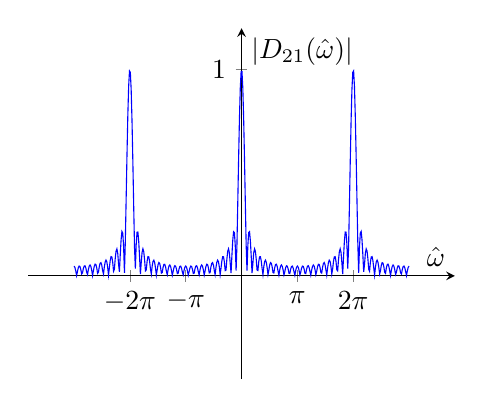
\begin{tikzpicture}
	\begin{axis}[width=7cm,
        domain=(-3*3.14):(3*3.14),
        samples=400,
        xmin=-12,
        xmax=12,
        ymin=-0.5,
        ymax=1.2,
    legend style={draw=none,at={(.99,.1)},anchor=south east},
        xlabel={$\hat{\omega}$},
	    ylabel={$|D_{21}(\hat{\omega})|$},
        axis x line=center, 
    axis y line=middle,
        ytick={0,1},
    xtick={-6.28,-3.14,0,3.14,6.28},
    xticklabels={$-2\pi$,$-\pi$,0,$\pi$,$2\pi$}    
    ]
    \addplot[blue] {abs(sin(deg(x*(10+0.50000001)))/(21*sin(1e-6+deg(x/2.0))))};
    \end{axis}
\end{tikzpicture}
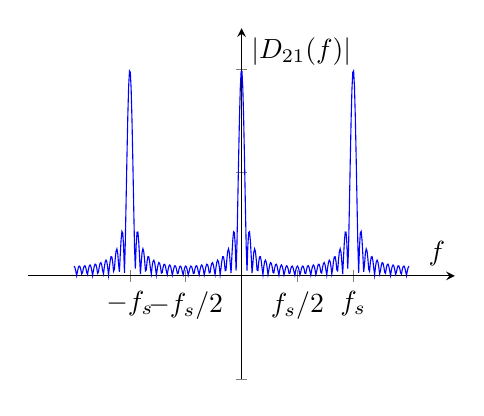
\begin{tikzpicture}
	\begin{axis}[width=7cm,
        domain=(-3*3.14):(3*3.14),
        samples=400,
        xmin=-12,
        xmax=12,
        ymin=-0.5,
        ymax=1.2,
    legend style={draw=none,at={(.99,.1)},anchor=south east},
        xlabel={$f$},
	    ylabel={$|D_{21}(f)|$},
        axis x line=center, 
    axis y line=middle,
            yticklabels={,,},
    xtick={-6.28,-3.14,0,3.14,6.28},
    xticklabels={$-f_s$,$-f_s/2$,0,$f_s/2$,$f_s$}    
    ]
    \addplot[blue] {abs(sin(deg(x*(10+0.50000001)))/(21*sin(1e-6+deg(x/2.0))))};
    \end{axis}
\end{tikzpicture}
\end{center}
\caption{A discrete-time Fourier transform is $2\pi$-periodic in frequency domain. The top figure shows the magnitude response of the running average filter $|D_{21}(\hat{\omega})|$ with frequency in units of radians per sample on the x-axis. Bottom: The same as the above, but with x-axis with frequency in units of cycles per second. The sampling-rate $f=\pm f_s/2$ corresponds to $\hat{\omega}=\pm \pi$.}
\label{fig:dir_kernelp}
\end{marginfigure}

The periodicity property is the same one that we encountered when
investigating aliasing of complex sinusoidal discrete-time signals,
which are essentially frequency components of a discrete-time
signal. Figure \ref{fig:dir_kernelp} shows one example of a
discrete-time Fourier transform, the Dirichlet kernel that we
encountered when investigating the frequency response of a running average filter. 

\section{Inverse transform}
The reverse operation is the inverse discrete-time Fourier transform,
which is defined as:
\begin{equation}
\boxed{
x[n] = \frac{1}{2\pi}\int_{-\pi}^{\pi} \hat{x}(\hat{\omega})e^{i\hat{\omega}n} d\hat{\omega}\,\,.
\label{eq:idtft_def}
}
\end{equation}
This allows transforming a discrete-time frequency domain
representation $\hat{x}(\hat{\omega})$ to a discrete-time signal $x[n]$.

It is quite easy to show that this inverse formula recovers $x[n]$ for
a DTFT $\hat{x}(\hat{\omega})$ that is defined as\sidenote{The inverse
transform is nearly the same as the Fourier series analysis equation
with $x[n]$ being the Fourier series coefficients and $\hat{x}(\hat{\omega})$ being a $2\pi$-periodic function.}:
\begin{equation}
\hat{x}(\hat{\omega}) = \sum_{n=-\infty}^{\infty} x[n] e^{-i\hat{\omega} n}\,\,,
\end{equation}
we can recover $x[n]$ using the inverse transform formula:
\begin{align}
\mathcal{F}^{-1}\left\{\hat{x}(\hat{\omega})\right\} &=\frac{1}{2\pi}\int_{-\pi}^{\pi} \hat{x}(\hat{\omega})e^{i\hat{\omega}n} d\hat{\omega} \\
     &=\frac{1}{2\pi}\int_{-\pi}^{\pi} \left[\sum_{m=-\infty}^{\infty} x[m]e^{-i\hat{\omega}m} \right] e^{i\hat{\omega}n} d\hat{\omega}\\
     &=\frac{1}{2\pi}\sum_{m=-\infty}^{\infty} \int_{-\pi}^{\pi} x[m]e^{i\hat{\omega}(n-m)} d\hat{\omega}\\
     &=\frac{1}{2\pi}\sum_{m=-\infty}^{\infty} 2\pi \delta[m-n] x[m]\\
     &=x[n]\qed
\end{align}
Here $\mathcal{F}^{-1}\{\cdot\}$ refers to the inverse DTFT.

We now have an inverse and forward discrete-time Fourier transform pair:
\begin{equation}
  \boxed{
    x[n] = \frac{1}{2\pi}\int_{-\pi}^{\pi} \hat{x}(\hat{\omega})e^{i\hat{\omega}n} d\hat{\omega} \xleftrightarrow{\mathcal{F}} 
    \hat{x}(\hat{\omega}) = \sum_{n=-\infty}^{\infty} x[n] e^{-i\hat{\omega}n}\,\,.
    }
\end{equation}
We'll now list several discrete-time Fourier transform pairs. Note
that many of these have in fact already been discussed in the chapter
for the continuous-time Fourier transform.

\if 0
\section{Frequency response for a real valued impulse response}

The frequency response of a real-valued impulse-response
$h[n]\in \mathbb{R}$ is conjugate symmetric
\begin{equation}
\boxed{
\He^* = \mathcal{H}(-\hat{\omega})\,\,.
}
\label{eq:conj_symmetry_lti}
\end{equation}
We can quite easily prove this:
\begin{align}
\He^* &= \left(\sum_k h[k] e^{-i\hat{\omega}k}\right)^* \\
        &= \sum_k h[k]^* e^{i\hat{\omega}k} \\
        &= \sum_k h[k] e^{i\hat{\omega}k} \\
        &= \mathcal{H}(-\hat{\omega})\,\,.
\end{align}
This follows from two facts: $(e^{i\phi})^* = e^{-i\phi}$ and $h[n]^*
= h[n]$.

We have already shown in the Fourier transform chapter that conjugate
symmetry is a more general property of the Fourier transform of real
valued signals. This is just a special case of this more general
property that is applied to discrete-time signals.

A corollary Equation \ref{eq:conj_symmetry_lti} of this is that the
magnitude response of an LTI system with a real valued impulse
response is always symmetric around zero:
\begin{equation}
\boxed{
|\He| = |\mathcal{H}(-\hat{\omega})|\,\,.
}
\end{equation}

\subsection{Example: real valued cosine and real valued impulse response}

Let's investigate the output of an LTI system with a real valued
impulse response $h[n]\in\mathbb{R}$ when the input signal is a real
valued cosine signal
\begin{equation}
x[n] = A\cos(\hat{\omega} n + \phi)\,\,.
\end{equation}
Using Euler's formula, we can express the input signal as a sum of a
positive and negative frequency complex sinusoidal signal:
\begin{equation}
x[n] = A \cos(\hat{\omega} n + \phi) = \frac{A}{2}e^{i\phi}e^{i\hat{\omega} n} + \frac{A}{2}e^{-i\phi}e^{-i\hat{\omega} n}\,\,.
\end{equation}
In this case, the output of the LTI system is:
\begin{align}
y[n] &= h[n]*x[n]\\
&= \sum_{k} h[k]x[n-k]\\
&= \sum_{k} h[k] \left( \frac{A}{2}e^{i\phi}e^{i\hat{\omega} (n-k)} + \frac{A}{2}e^{-i\phi}e^{-i\hat{\omega} (n-k)} \right)\\
 &= \left(\sum_{k} h[k] e^{-i\hat{\omega} k}\right) \frac{A}{2}e^{i\phi}e^{i\hat{\omega} n} + \left(\sum_{k} h[k] e^{i\hat{\omega} k}\right) \frac{A}{2}e^{-i\phi} e^{-i\hat{\omega} n}\\
 &= \mathcal{H}(\hat{\omega}) \frac{A}{2}e^{i\phi}e^{i\hat{\omega} n} + \mathcal{H}(-\hat{\omega}) \frac{A}{2}e^{-i\phi}e^{-i\hat{\omega} n}\,\,.
 \end{align} 
In this case, the impulse response is real valued $h[n]\in \mathbb{R}$, and thus:
\begin{equation}
\mathcal{H}(-\hat{\omega}) = \mathcal{H}(\hat{\omega})^*\,\,.
\end{equation}
This means that we can write the output signal as a sum:
\begin{align}
y[n] &= \He \frac{A}{2}e^{i\phi}e^{i\hat{\omega} n} +  \He^*\frac{A}{2}e^{-i\phi} e^{-i\hat{\omega} n}\,\,.
\end{align}
Which means that the spectral components are conjugate symmetric. The output of the real valued sinusoidal signal is then:
\begin{align}
y[n] &= |\He|\frac{A}{2} e^{i(\phi + \angle \He)}e^{i\hat{\omega} n} + |\He|\frac{A}{2}e^{-i(\phi + \angle \He)} e^{-i\hat{\omega} n} \\
 & = |\He| A \cos(\hat{\omega} n + \phi + \angle \He)\,\,.
\end{align}
The output signal is a cosine signal with the same frequency as the
input signals. The amplitude is scaled with the magnitude response
$|\He|$ and the phase is shifted by $\angle \He$.

\fi




\usetikzlibrary{arrows.meta, positioning, quotes}
\begin{marginfigure}
 \begin{center}
 \begin{tikzpicture}[
    node distance=5mm and 20mm,
    box/.style = {draw, minimum height=12mm, align=center},
    sy+/.style = {yshift= 2mm}, 
    sy-/.style = {yshift=-2mm},
    every edge quotes/.style = {align=center}
                        ]    
\node (n1) [box]             {$h[n]$\\Time domain};                        
\node (n2) [box,right=of n1] {$\He$\\Frequency domain};
%
\draw[thick,-Triangle]  
    ([sy+] n1.east) to [above] ([sy+] n2.west);
\draw[thick,-Triangle, dashed]  
    ([sy-] n2.west) -- ([sy-] n1.east);
    \end{tikzpicture}
\end{center}
\caption{The frequency response $\He$ of an LTI system is the Fourier transform of the impulse response $h[n]$.}
\end{marginfigure}

\section{Frequency response}

The frequency response of a discrete-time LTI system (shown earlier in Equation \ref{eq:dt_fr}) 
\begin{equation}
\He = \sum_{k=-\infty}^{\infty} h[k] e^{-i\hat{\omega} k}
\end{equation}
is a discrete-time Fourier transform of the impulse response
$h[n]$. This means that all the properties of a discrete-time Fourier
transform will apply also to a frequency response. Using our short
hand notation, we can define this as a DTFT pair:
\begin{equation}
\boxed{
h[n] \xleftrightarrow{\mathcal{F}} \He\,\,.
}
\end{equation}
The inverse DTFT formula will come in handy when e.g., defining LTI
systems based on their frequency response characteristics, and then
obtaining the impulse response using the inverse transform. This leads
to e.g., ideal filters, ideal frequency selective filters, and
arbitrary time shift filters. These are LTI systems that would be
difficult or impossible to derive in time domain.

\section{Time-shifted unit impulse}

DTFT for unit impulse is:
\begin{equation}
\boxed{
x[n] = \delta[n-n_0] \xleftrightarrow{\mathcal{F}} \hat{x}(\hat{\omega}) = e^{-i\hat{\omega}n_0}\,\,.
}
\end{equation}
The proof is trivial. 

\section{Frequency shift $e^{i\hat{\omega}_0n}x[n]$}

A shift in frequency domain corresponds to multiplication
by a complex exponential signal in time domain.  If
\begin{equation}
x[n] \xleftrightarrow{\mathcal{F}} \hat{x}(\hat{\omega})\,\,,
\end{equation}
then
\begin{equation}
\boxed{
e^{i\hat{\omega}_0 n}x[n] \xleftrightarrow{\mathcal{F}} \hat{x}(\hat{\omega}-\hat{\omega}_0)\,\,.
}
\end{equation}
The proof is as follows. If we multiply the signal $x[n]$ with a
complex exponential signal with frequency $\hat{\omega}_0$ we obtain a
new signal $y[n]$:
\begin{equation}
y[n] = e^{i\hat{\omega}_0 n}x[n]\,\,. 
\end{equation}
If we DTFT this, we obtain:
\begin{align}
\hat{y}(\hat{\omega})&=\sum_{k=-\infty}^{\infty} e^{i\hat{\omega}_0 k}x[k]e^{-i\hat{\omega}k} \\
&=\sum_{k=-\infty}^{\infty} x[k] e^{-i(\hat{\omega}-\hat{\omega}_0)k} = \hat{x}(\hat{\omega}-\hat{\omega}_0)\qed\,\,.
\end{align}
Multiplying a time domain signal by a complex sinusoid with frequency
$\hat{\omega}_0$ results in a frequency shift of the signal in
frequency domain.

This property is useful for creating a filter with a specific center
frequency. This property can also be used to shift the center
frequency of a signal in frequency domain, e.g., in digital up or
downconversion systems that are found in digital radios.

\section{Convolution theorem}
An often used theorem of signal processing is the convolution theorem. It
states that convolution in time domain is multiplication in frequency
domain. This is also applies to discrete-time Fourier transforms.
\begin{equation}
\boxed{
a[n] = b[n]*c[n] \xleftrightarrow{\mathcal{F}} \hat{a}(\hat{\omega}) = \hat{b}(\hat{\omega})\hat{c}(\hat{\omega})\,\,.
}
\end{equation}
The proof is identical to the proof shown in the chapter on Fourier transforms.

\begin{marginfigure}

\begin{center}
  \begin{tikzpicture}[node distance=3cm,auto,>=latex']

    \node [int] (a) {LTI $(h_1[n])$};
    \node [above of=a, node distance=1cm] (in) {$x[n]$};
    \node [int, below of=a, node distance=1cm] (b) {LTI $(h_2[n])$};
    \node [below of=b, node distance=1cm] (out) {$y[n]$};
    \path[->] (a) -> (b);
    \draw[->] (a) -> (b);
    \path[->] (in) -> (a);
    \draw[->] (in) -> (a);
    \path[->] (b) -> (out);
    \draw[->] (b) -> (out);
    
    \node [int, right of=a,node distance=2cm] (a3) {LTI $(h_3[n])$};
    \node [above of=a3, node distance=1cm] (in3) {$x[n]$};
    \node [below of=a3, node distance=1cm] (out3) {$y[n]$};
    \path[->] (in3) -> (a3);
    \draw[->] (in3) -> (a3);
    \path[->] (a3) -> (out3);
    \draw[->] (a3) -> (out3);
    
\end{tikzpicture}
\end{center}
\caption{A consequence of the associative property of convolution is
  that two LTI systems characterized with $h_1[n]$ and $h_2[n]$ can be
  combined as a single LTI system with impulse response
  $h_3[n]=h_1[n]*h_2[n]$. The convolution theorem allows us to
  investigate the combined frequency response of the system using the following formula:
  $\mathcal{H}_3(\hat{\omega})=\mathcal{H}_1(\hat{\omega})\mathcal{H}_2(\hat{\omega})$.}
\label{fig:cascade_lti}
\end{marginfigure}


\subsection{Example: cascaded filters}

A consequence of the convolution theorem is that we can analyze the
combined effect of a cascaded system, simply by multiplying together
the frequency responses.

Let's assume that a signal is first convolved with a filter that has
an impulse response $h_1[n]$ and then with a filter that has an
impulse response $h_2[n]$:
\begin{align}
  y[n] &= h_2[n]*(h_1[n]*x[n])\\
  &= (h_1[n]*h_2[n])*x[n]\\
  &= h_3[n]*x[n]\,\,.
\end{align}
The combined frequency response $\mathcal{H}_3(\hat{\omega})$ of the
cascaded system is $\mathcal{H}_1(\hat{\omega})\mathcal{H}_2(\hat{\omega})$:
\begin{equation}
  \boxed{
    h_3[n]=h_1[n]*h_2[n] \xleftrightarrow{\mathcal{F}} \mathcal{H}_3(\hat{\omega}) = \mathcal{H}_1(\hat{\omega})\mathcal{H}_2(\hat{\omega})
    }
\end{equation}
where $\mathcal{H}_1(\hat{\omega})$ and $\mathcal{H}_2(\hat{\omega})$
are the frequency responses corresponding to impulse responses
$h_1[n]$ and $h_2[n]$.

\if 0
\subsection*{Proof}
Consider the convolution of two signals $a[n]$ and $b[n]$:
\begin{align}
Y(e^{i\hat{\omega}}) = a[n]*b[n] = \sum_k a[k] b[n-k]\,\,.
\end{align}
The discrete-time Fourier transform of these signals is:
\begin{align}
Y(e^{i\hat{\omega}}) &= \sum_n (a[n]*b[n]) e^{-i\hat{\omega}n}\\
     &= \sum_n \left(\sum_k a[k]b[n-k]\right) e^{-i\hat{\omega}n}\\
     &= \sum_k a[k] \left(\sum_n b[n-k] e^{-i\hat{\omega}n}\right)\,\,.
\end{align}
If we now do a variable substitution: $n-k=\ell$, we obtain:
\begin{align}
Y(e^{i\hat{\omega}}) &= \sum_k a[k] \left(\sum_\ell b[\ell] e^{-i\hat{\omega}(\ell+k)}\right)\\
     &= \left(\sum_k a[k] e^{-i\hat{\omega}k}\right) \left(\sum_\ell b[\ell] e^{-i\hat{\omega}\ell}\right)\\
     &= A(e^{i\hat{\omega}})B(e^{i\hat{\omega}})\,\,.
\end{align}
This means that convolution is equivalent to multiplication in frequency domain. 

\subsection*{Alternate proof}

A convolution is defined as:
\begin{align}
    y[n] &= a[n] * b[n]\\
    &= \sum_k a[k] b[n-k]\,\,.
\end{align}
Now we know that $a[n]$ and $b[n]$ have a discrete-time Fourier transform representation:
\begin{align}
    A(e^{i\hat{\omega}}) &= \sum_k a[k] e^{-i\hat{\omega}k}\\
    B(e^{i\hat{\omega}}) &= \sum_k b[k] e^{-i\hat{\omega}k}\,\,.
\end{align}
and inverse discrete-time Fourier transforms:
\begin{align}
    a[n] &= \frac{1}{2\pi}\int_{-\pi}^{\pi}A(e^{i\hat{\omega}})e^{i\hat{\omega}n}d\hat{\omega}\\
    b[n] &= \frac{1}{2\pi}\int_{-\pi}^{\pi}B(e^{i\hat{\omega}})e^{i\hat{\omega}n}d\hat{\omega}\,\,.
\end{align}
If we insert $b[n]$ as a function of $B(e^{i\hat{\omega}})$ into the convolution equation, we get
\begin{align}
    y[n] &= \sum_k a[k]\frac{1}{2\pi}\int_{-\pi}^{\pi}B(e^{i\hat{\omega}})e^{i\hat{\omega}(n-k)}d\hat{\omega}\\
     &= \frac{1}{2\pi}\int_{-\pi}^{\pi}\left(\sum_k a[k] e^{-i\hat{\omega}k} \right)B(e^{i\hat{\omega}})e^{i\hat{\omega}n}d\hat{\omega}\\
 &= \frac{1}{2\pi}\int_{-\pi}^{\pi}A(e^{i\hat{\omega}})B(e^{i\hat{\omega}})e^{i\hat{\omega}n}d\hat{\omega}\,\,.
\end{align}
We can again see that convolution is multiplication in frequency domain.
\fi 


